\documentclass{article}
\usepackage[utf8]{inputenc}
\usepackage{multicol}
\usepackage[formats]{listings}
\lstloadaspects{formats}
\usepackage{verbatim}
\usepackage{color}
\usepackage{geometry}
\usepackage{float}
\usepackage{amsmath}
\usepackage{multirow}% http://ctan.org/pkg/multirow
\usepackage{hhline}% http://ctan.org/pkg/hhline
\usepackage{caption}
\usepackage{pdflscape}
\usepackage{caption}
\usepackage[font={color=black},figurename=Fig.,labelfont={it}]{caption}
\usepackage{hyperref}
\setlength{\belowcaptionskip}{-10pt}
\setlength{\abovecaptionskip}{-30pt}
\floatstyle{boxed} 
\restylefloat{figure}
\usepackage{graphicx}
\usepackage{subcaption}
\definecolor{codegreen}{rgb}{0,0.6,0}
\definecolor{codegray}{rgb}{0.5,0.5,0.5}
\definecolor{codepurple}{rgb}{0.58,0,0.82}
\definecolor{backcolour}{rgb}{0.95,0.95,0.92}
\lstdefinestyle{mystyle}{
	backgroundcolor=\color{backcolour},   
	commentstyle=\color{codegreen},
	keywordstyle=\color{blue},
	numberstyle=\tiny\color{codegray},
	stringstyle=\color{codepurple},
	basicstyle=\footnotesize,
	breakatwhitespace=false,         
	breaklines=true,                 
	captionpos=b,                    
	keepspaces=true,                 
	numbers=left,                    
	numbersep=5pt,                  
	showspaces=false,                
	showstringspaces=false,
	showtabs=false,                  
	tabsize=2
}
\lstset{style=mystyle}
\title{Data Mining\\
		Home work 12\\Clustering, PCA, OLAP}
\author{Aqeel Labash\\ \textbf{Lecturer:} Jaak Vilo}
\geometry{
	a4paper,
	total={170mm,257mm},	
	left=10mm,
	top=5mm,
}
\begin{document}
	\maketitle
\section*{First Question}
For this question I tried K-means. I used the following code : 
\begin{lstlisting}[language=Python]
import numpy as np
import pandas as pd
from sklearn.cluster import KMeans
with open ('DM2016_org.txt') as f:
    d = {}
    headers = f.readline().split(' ')
    values = map(lambda x:x.split(),f.readlines())
    for i in range(len(values[0])):
        d[i]=[]
        for v in values:
            d[i].append(v[i])
data = pd.DataFrame(d)
npdata = data[data.columns[1:]].as_matrix()
npdata = np.array(npdata,dtype=int)
random_state = 170
nc = 339
y_pred = KMeans(n_clusters=nc, random_state=random_state,precompute_distances=True).fit_predict(npdata)
output=[]
for i in range(nc):
    print i
    map(lambda x:output.append(x),map(lambda x:data[data.index[0]][x].values,np.where(y_pred==i))[0])
f = open('Kmeans_399.txt','w')
for element in output:
    f.write('\n{}'.format(element))
f.close()
\end{lstlisting}
I tried 3 values as number of clusters 2,10,30,399. The results were as following:
\begin{figure}[H]
\begin{subfigure}{.5\textwidth}
  \centering

\includegraphics[scale=0.15]{kmeans_2.png}
  \caption{KMeans 2 clusters}
  \label{fig:sfig1}
\end{subfigure}
\begin{subfigure}{.5\textwidth}
  \centering

\includegraphics[scale=0.15]{kmeans_10.png}
  \caption{KMeans 10 clusters}
  \label{fig:sfig2}
\end{subfigure}

\begin{subfigure}{.5\textwidth}
\vspace{5mm}
  \centering

\includegraphics[scale=0.15]{kmeans_30.png}
  \caption{KMeans 30 clusters}
  \label{fig:sfig3}
  \vspace{5mm}
\end{subfigure}
\begin{subfigure}{.5\textwidth}
\vspace{5mm}
  \centering

\includegraphics[scale=0.15]{kmeans_399.png}
  \caption{KMeans 30 clusters}
  \label{fig:sfig4}
  \vspace{5mm}
\end{subfigure}
\caption{Shows Comparsion between different number of clusters using K-Means}
\end{figure}
Only getting a cluster values won't work because in that case we only know the cluster elements.Which won't let us know the order of the cluster. That information is crucial in our case.\\
After that I tried hierarchical clustering using Scipy library. The full size dendogram was as following :
\newgeometry{
 	a4paper,
 	total={170mm,257mm},	
 	left=0mm,
 	top=10mm,
 	right=0mm,
 	bottom=0mm
 }
\begin{landscape}

\begin{figure}[H]
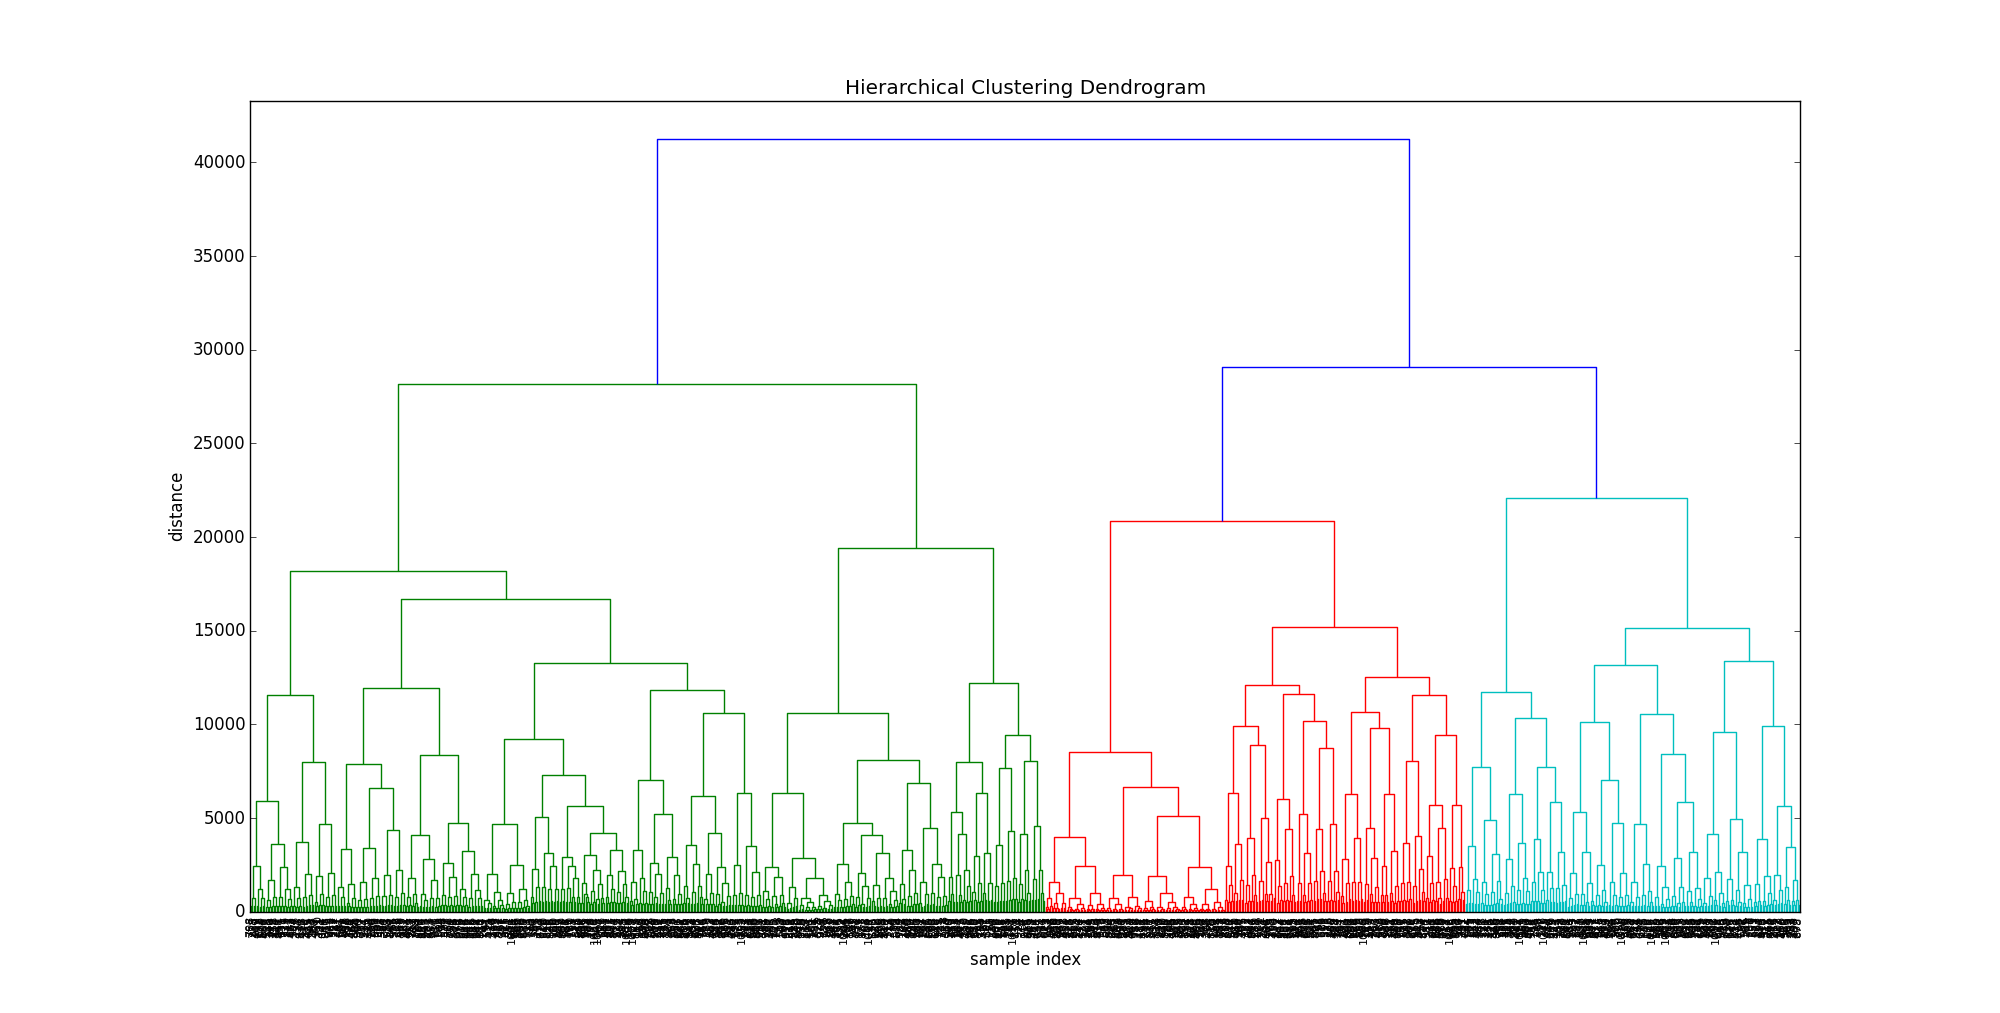
\includegraphics[scale=0.7,trim={4cm 1cm 5cm 2cm},clip]{dendogram_full.png}
\caption{Full dendogram}
\end{figure} 

\begin{figure}[H]
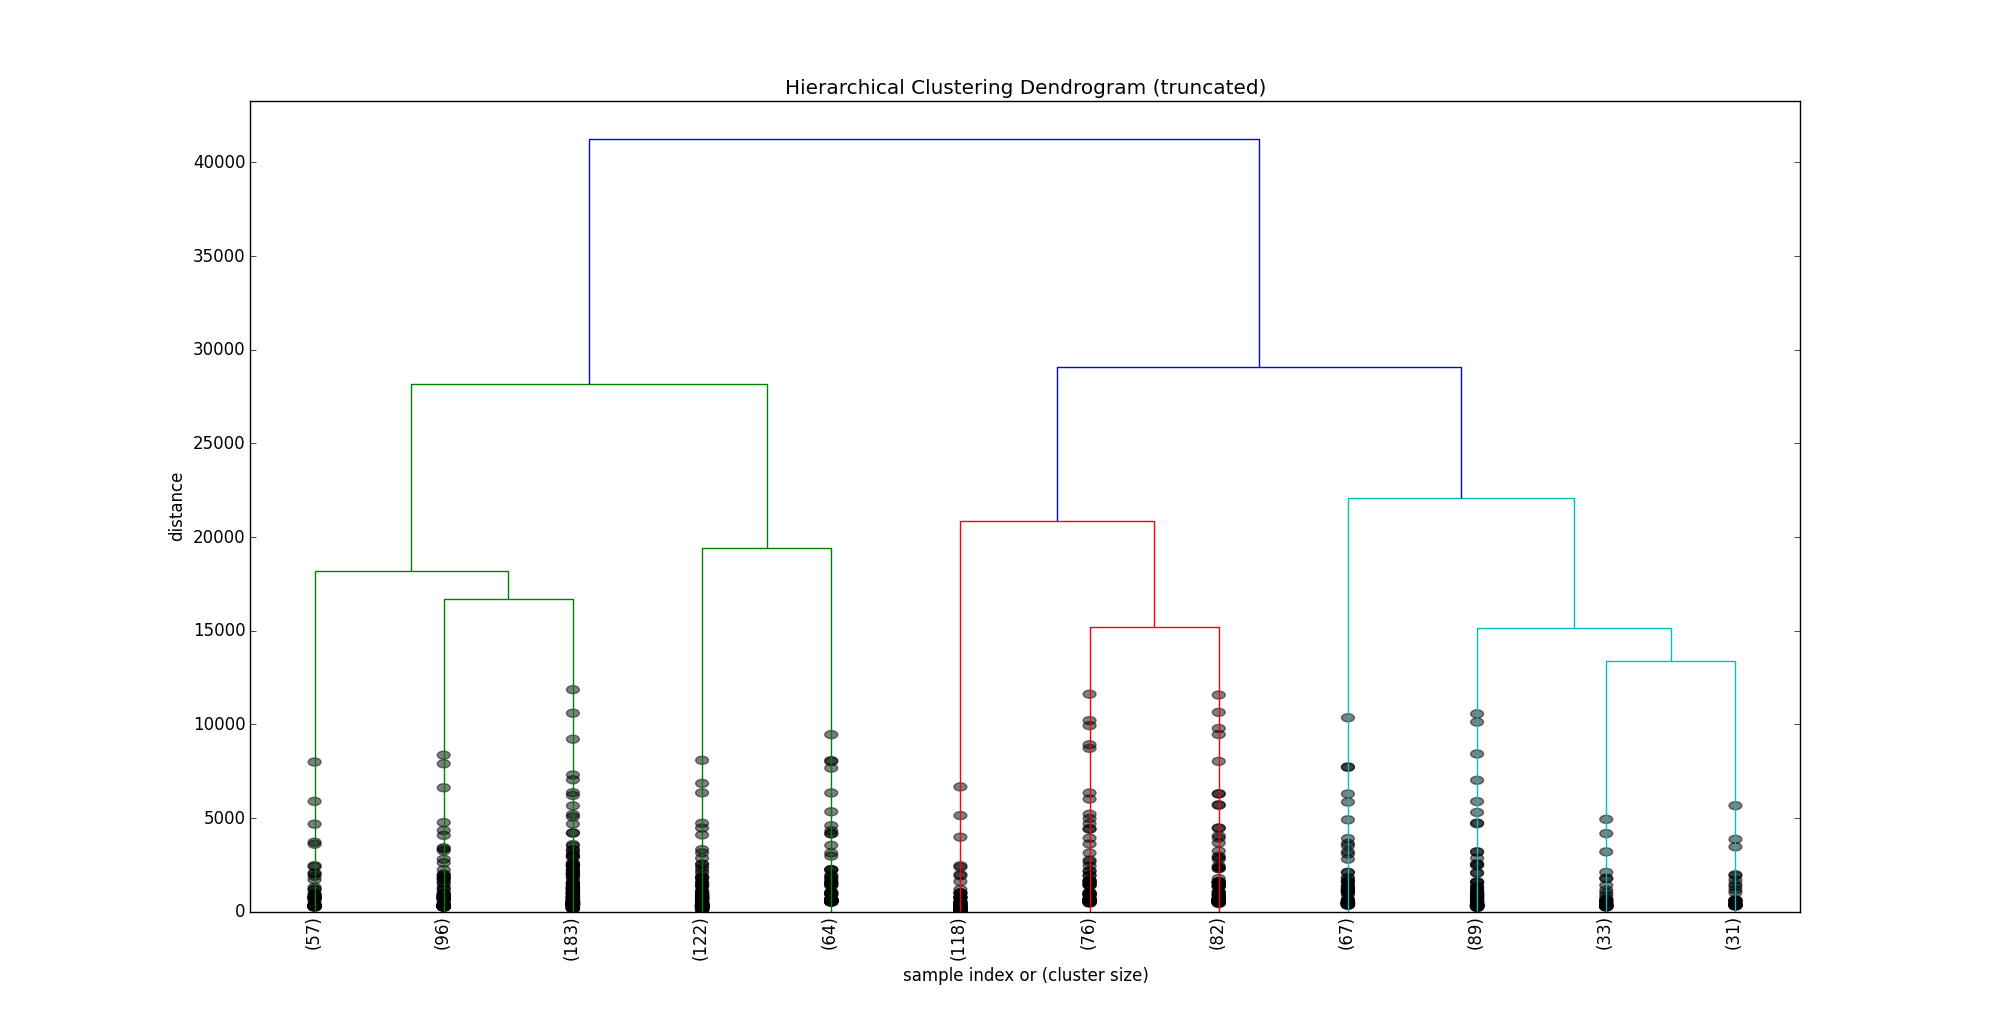
\includegraphics[scale=0.69,trim={4cm 0cm 5cm 2cm},clip]{dendogram_truncated_clustersize.png}
\caption{Truncated Dendogram}
\end{figure} 
\end{landscape}
\newgeometry{
	a4paper,
	total={170mm,257mm},	
	left=10mm,
	top=5mm,
}
\section*{Second Question}
For this question I read the file in python and extract the data as matrix and then used sklearn for PCA and used matplotlib for 3d plotting. Here is the code :
\begin{lstlisting}[language=Python]
import numpy as np
from sklearn.decomposition import PCA
import pandas as pd
import matplotlib.pyplot as plt
from mpl_toolkits.mplot3d import Axes3D
with open ('DM2016_org.csv') as f:
    d = {}
    headers = f.readline().split(' ')
    values = map(lambda x:x.split(),f.readlines())
    for i in range(len(values)):
        d[headers[i]]=[]
        for v in values:
            d[headers[i]].append(v[i])
data = pd.DataFrame(d)
npdata = data[data.columns[1:]].as_matrix()
pca = PCA(n_components=3)
pca.fit(npdata)
output = pca.transform(npdata)
fig = plt.figure()
ax = fig.add_subplot(111, projection='3d')
n = 100
for x, y, z in output:
    ax.scatter(x, y, z)

ax.set_xlabel('X Label')
ax.set_ylabel('Y Label')
ax.set_zlabel('Z Label')

plt.show()
\end{lstlisting}
And here is the output figure:
\begin{figure}[H]
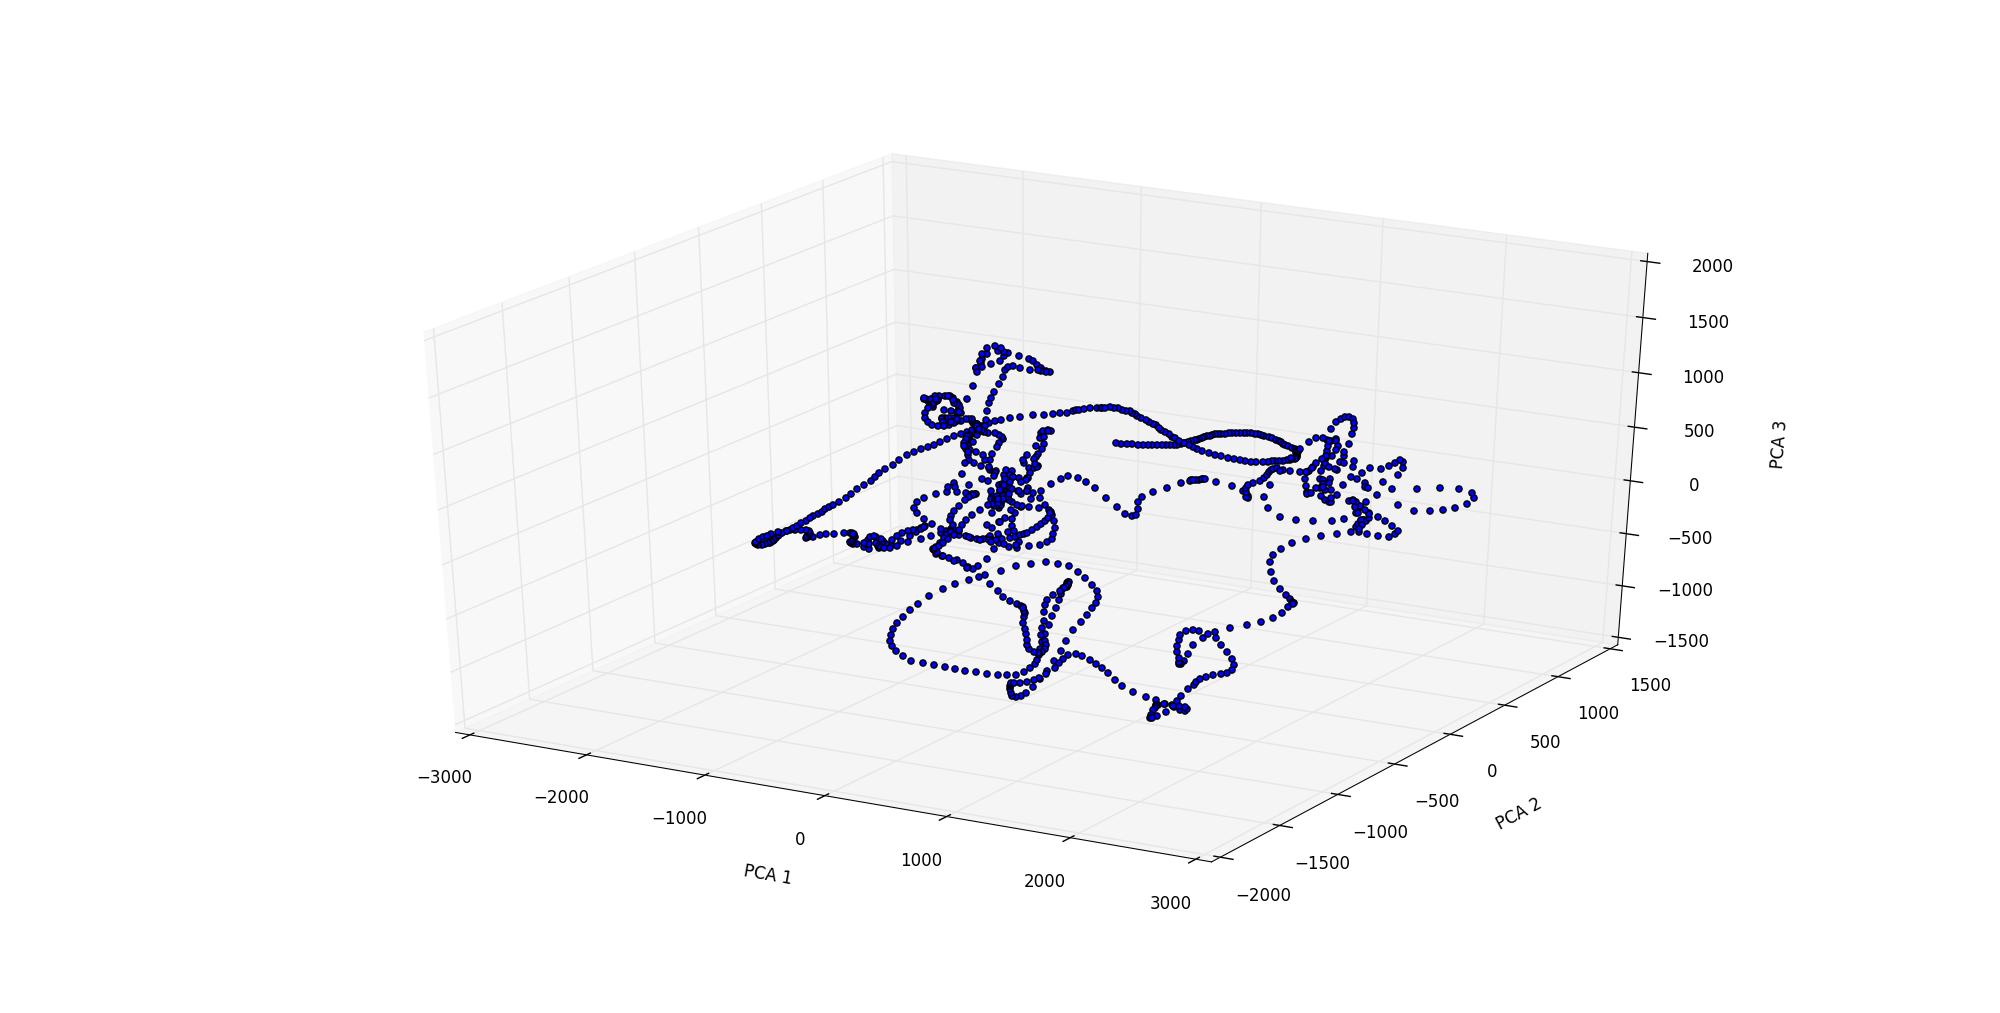
\includegraphics[scale=0.5,trim={8cm 2cm 10cm 5cm},clip]{3D.png}
\caption{X: PCA1 , Y:PCA2 , Z:PCA3}
\end{figure}
\section*{Third Question}
For this question I used the following code to find pivot table on basis of Gender and education :
\begin{lstlisting}[language=Python]
import pandas as pd
import numpy as np
%matplotlib inline
import matplotlib.pyplot as plt
data = pd.read_csv('extract_medium.csv',sep=';')
data.head(1)
table = pd.pivot_table(data,values='Earnings',index=['Sex', 'Education'],aggfunc=np.mean)
##OR###
temp1 = data.groupby(['Sex', 'Education']).Earnings.mean()
temp1
temp1 = temp1.values
test=temp1.reshape(2,17)
test.shape
plt.pcolor(test,cmap=plt.cm.Reds,vmin=np.min(test), vmax=np.max(test))
plt.yticks([0,1],range(3))
plt.xticks(range(17),range(17))
plt.title('Heat map of average Earnings Gender Vs Education')
plt.show()
plt.close()
\end{lstlisting}
And here is the pivot table : 
\begin{table}[H]
  \centering
  \begin{tabular}{|c|c|c|}
  \hline
    Sex&Education&Average earning\\ \hline
    \multirow{16}{*}{Male}&Not in universe (Under 3 years)&0.000000\\ \hhline{~--} 
	&No schooling completed&3504.784689\\ \hhline{~--}
	&Nursery school to 4th grade&690.859232\\ \hhline{~--}
	&5th or 6th grade&5083.671988\\ \hhline{~--}
	&7th or 8th grade&4073.961606\\ \hhline{~--}
	&9th grade&9596.498516\\ \hhline{~--}
	&10th grade&11185.848485\\ \hhline{~--}
	&11th grade&11167.638889\\ \hhline{~--}
	&12th grade,no diploma&19404.356436\\ \hhline{~--}
	&High school graduate&24012.275826\\ \hhline{~--}
	&college,less than 1 year&28201.210614\\ \hhline{~--}
	&college 1+ years, no degree&28488.347335\\ \hhline{~--}
	&Associate degree&35081.001821\\ \hhline{~--}
	&Bachelor,s degree&53294.264282\\ \hhline{~--}
	&Master.s degree&70755.173611\\ \hhline{~--}
	&Professional degree&94245.204918\\ \hhline{~--}
	&Doctorate degree&61467.676768 \\\hline
    \multirow{16}{*}{Female}&Not in universe (Under 3 years)&0.000000\\ \hhline{~--}
	 &No schooling completed&947.790323\\ \hhline{~--} 
	 &Nursery school to 4th grade&387.342995\\ \hhline{~--} 
	 &5th grade or 6th grade&2771.055195\\ \hhline{~--} 
	 &7th or 8th grade&2256.137405\\ \hhline{~--} 
	 &9th grade&3326.657609\\ \hhline{~--} 
	 &10th grade&4281.338798\\ \hhline{~--} 
	 &11th grade&5003.164557\\ \hhline{~--} 
	 &12th grade,no diploma&9200.885781\\ \hhline{~--} 
	 &High school graduate&11515.832571\\ \hhline{~--} 
	 &college,less than 1 year&16305.045514\\ \hhline{~--} 
	 &college 1+ years, no degree&16949.317489\\ \hhline{~--} 
	 &Associate degree&21991.480263\\ \hhline{~--} 
	 &Bachelor,s degree&33193.713496\\ \hhline{~--} 
	 &Master.s degree&44412.231834\\ \hhline{~--} 
	 &Professional degree&46821.961290\\ \hhline{~--} 
	 &Doctorate degree&41476.065574 \\ \hline
  \end{tabular}
  \label{T:peak}
\end{table}
And here is the heatmap : 
\begin{figure}[H]
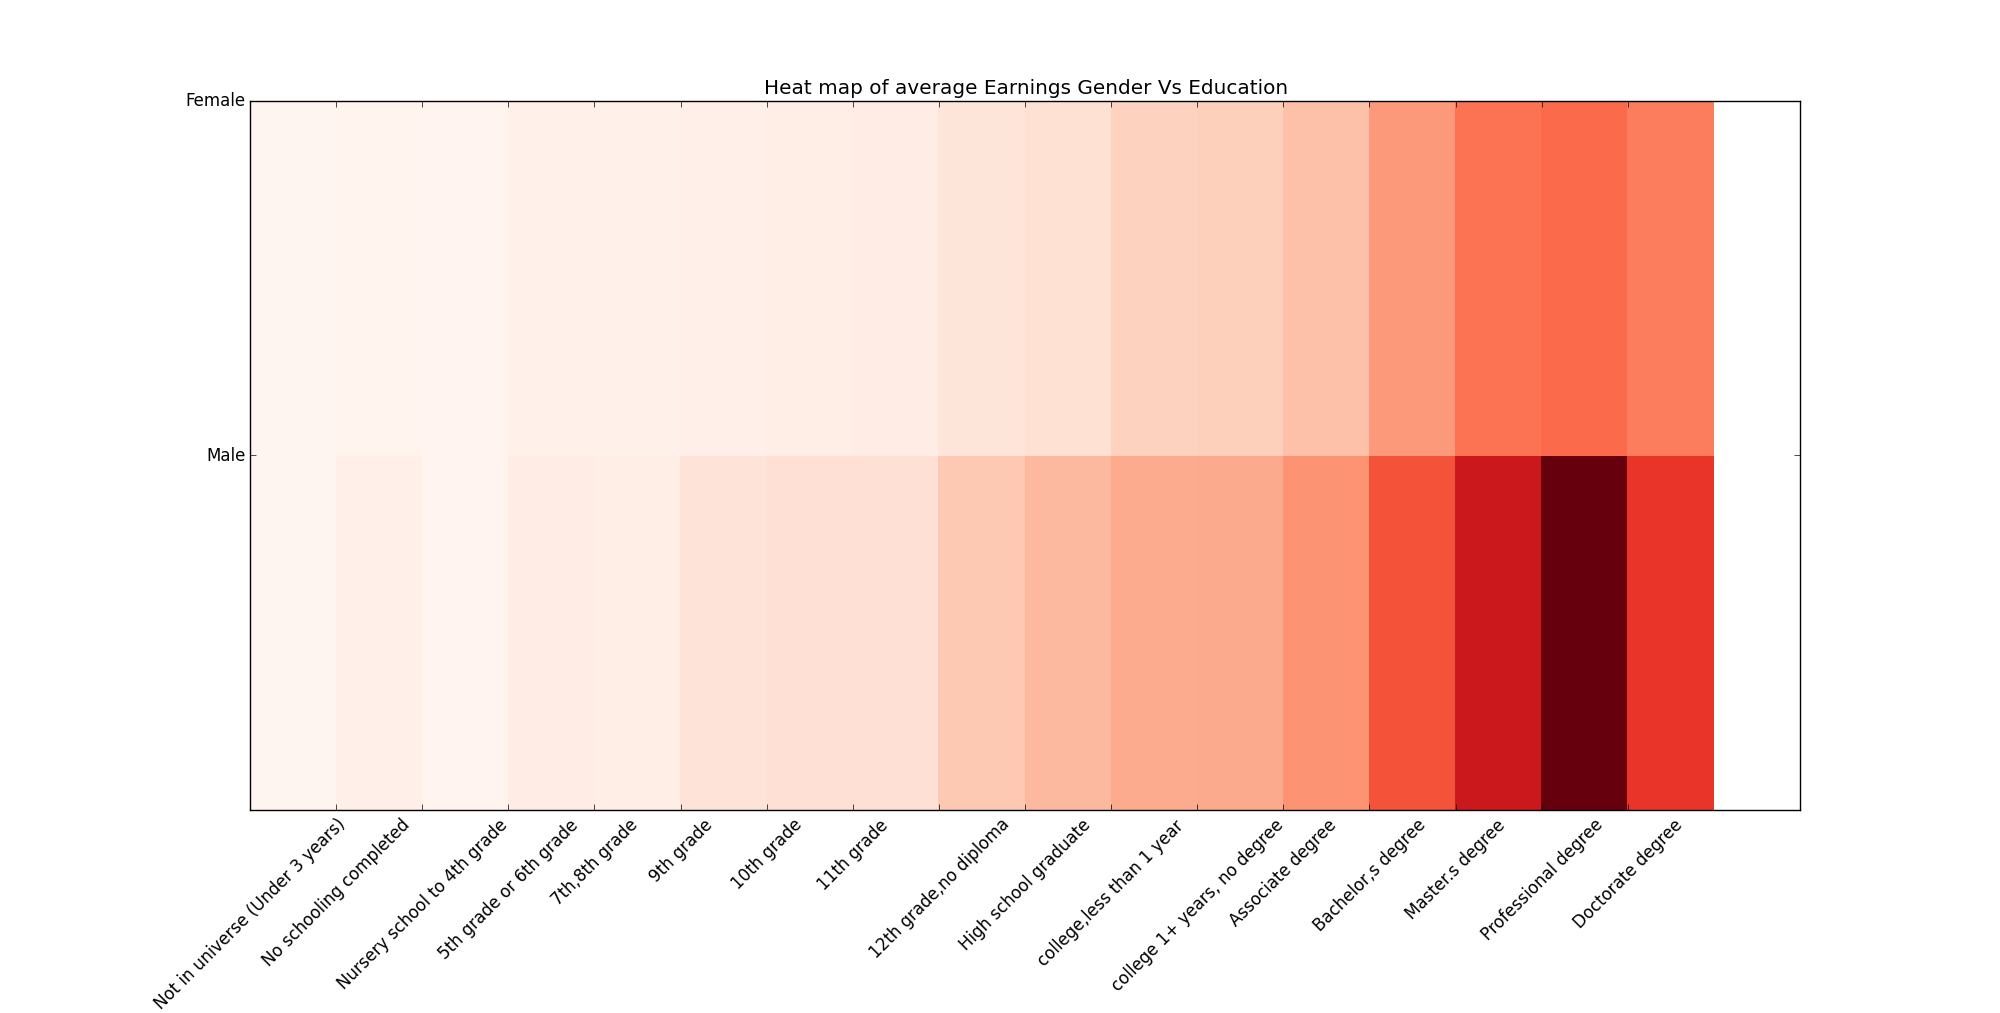
\includegraphics[scale=0.42,trim={3cm 0cm 7cm 2cm},clip]{hmGEE.png}
\caption{Heatmap gender vs education in earnings}
\end{figure}
It's really cool. Have profissinoal degree or master is better than have a doctoral. I think that's because most doctoral degree work in education which is not the highest salaries.
\section*{Fourth Question}
For this question I will show the relation between marital status , gender and earnings seemed interesting :) and here is the code : 
\begin{lstlisting}[language=python]
table = pd.pivot_table(data,values='Earnings',index=['Sex', 'Marriage'],aggfunc=np.mean)
table = table.values
test=table.reshape(2,5)
fig = plt.figure()
ax = fig.add_subplot(111)
ax.pcolor(test,cmap=plt.cm.Reds,vmin=np.min(test), vmax=np.max(test))
ax.set_yticks([1,2])
ax.set_yticklabels(Genders)
ax.set_xticks(range(6))
ax.set_xticklabels(MarriageState)
for tick in ax.get_xticklabels():
    tick.set_rotation(45)
plt.gcf().subplots_adjust(bottom=0.20)
ax.set_title('Heat map of average Earnings Gender Vs Mariage')
plt.show()
plt.close()
\end{lstlisting}
The resulted heat map :
\begin{figure}[H]
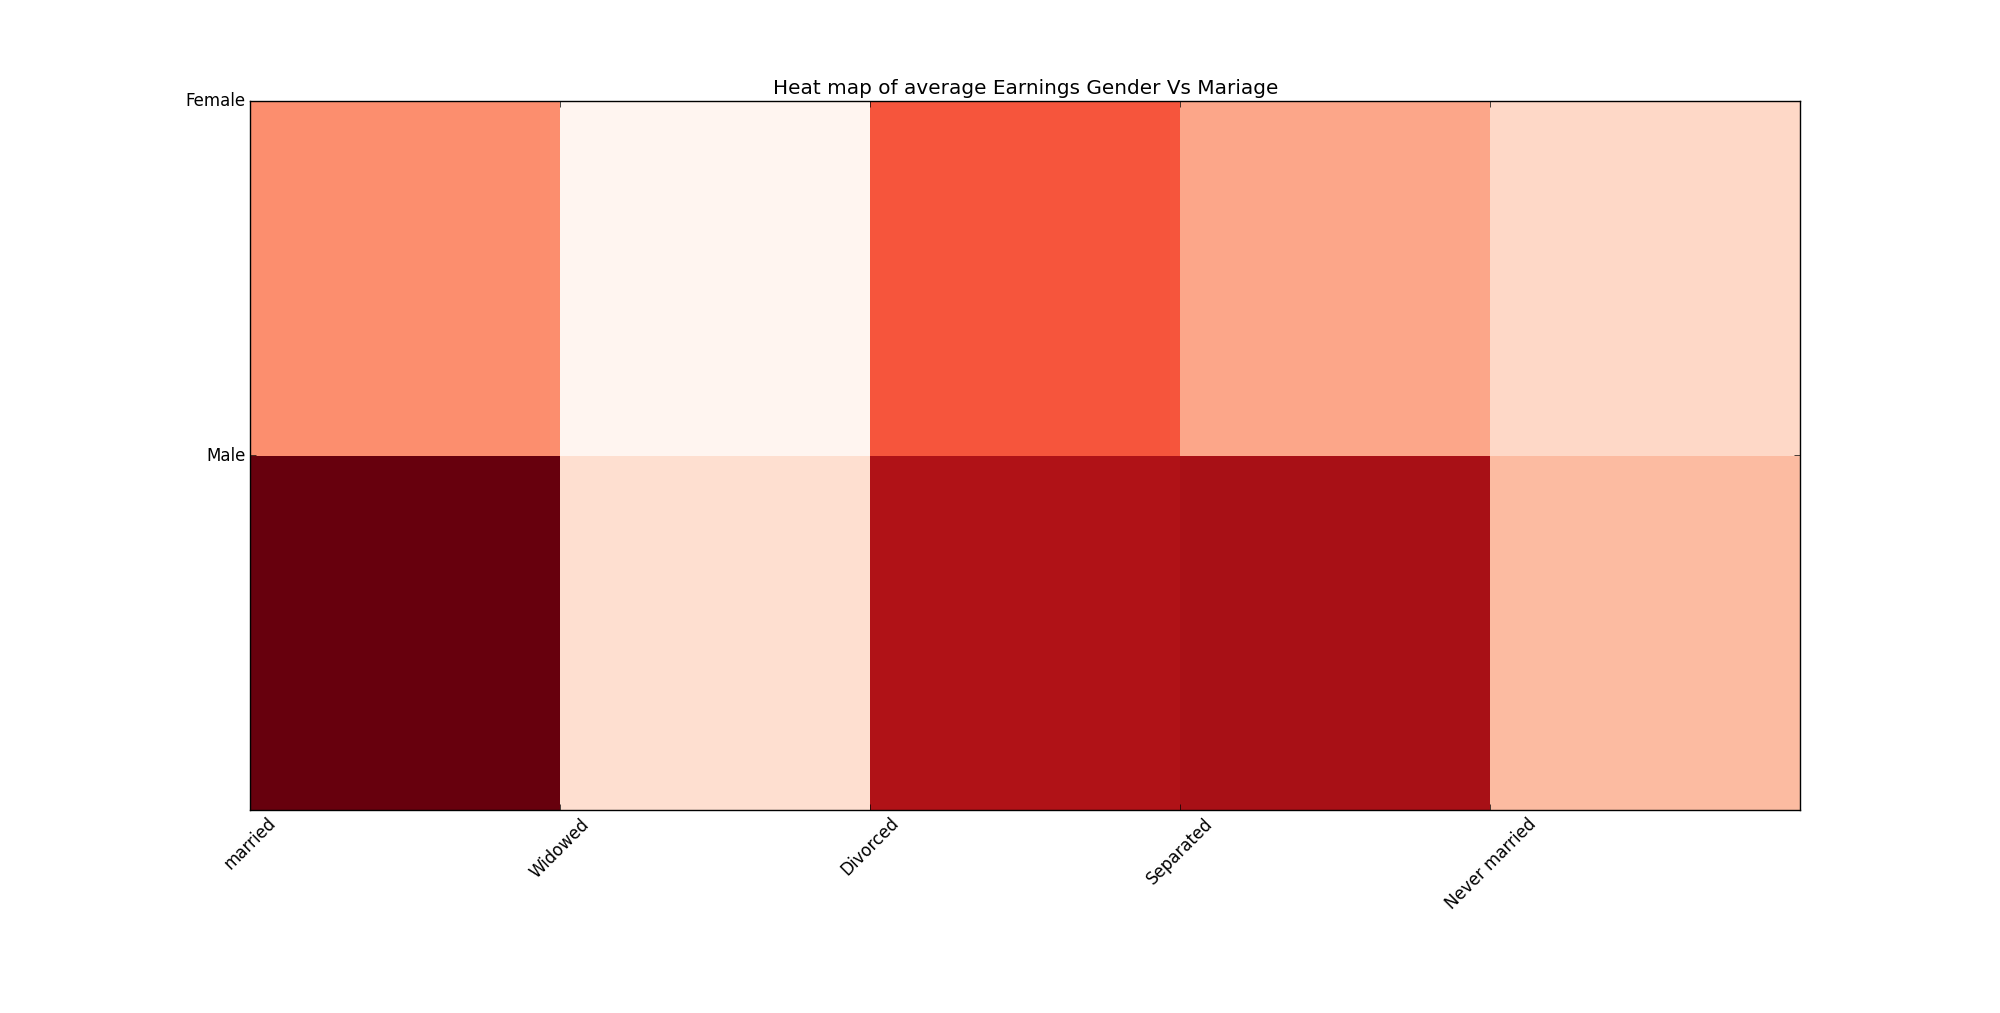
\includegraphics[scale=0.4,trim={4cm 2.5cm 0cm 2cm},clip]{hmGME.png}
\caption{Heatmap gender vs marriage status in earnings}
\end{figure}
depending on this data if you want to increase your earning just get married :D but don't kill your partner that will decrease your income dramatically.
\section*{Fifth Question}
I did read most of the article but the operation were quite more understandable and clear on the wikipedia web page.
For this task I'll aggregate (Sex,Marriage,Hours) as (X,Y,Z) please notice that Y we can convert it to days -> weeks depending on the value we have.
The operations are : 
\begin{enumerate}
\item \textbf{Slicing}: by this we can take one males or females.
\item \textbf{Dicing}: by this we can take group of hours (or group of days if we generalize this value).
\item \textbf{Drill-up and drill-down}:let's say Hours is genralized to days and we can generalize it to weeks and currently we are using days.At this point drill down will go to Hours for specific values and Drill-up will generalize to weeks.
\item \textbf{Pivoting}: is about changing axes like changing axes between sexes and hours.
\end{enumerate}
To calculate the data cube I used the following code \\ 
\textbf{Note:}The following code depending on the previous code.
\begin{lstlisting}[language=Python]
table = pd.pivot_table(data,values='Earnings',index=['Sex', 'Marriage','Hours'],aggfunc=np.mean)
\end{lstlisting}
The previous code will calculate the required data pivot but I could not find a good way to show interactive plot.

I hope I understood the question.
\section*{Sixth Question}
For this question I used python as usual and used google TSP to increase the speed and performance. (even though it's not a straight forward solution). Here is the code : 
\begin{lstlisting}[language=Python]
__author__ = 'Modified by :aqeel'
import pandas as pd
import numpy as np
import RandomMatrix
import ShortestPathFinder
# Copyright 2010-2014 Google
# Licensed under the Apache License, Version 2.0 (the "License");
# you may not use this file except in compliance with the License.
# You may obtain a copy of the License at
#
#     http://www.apache.org/licenses/LICENSE-2.0
#
# Unless required by applicable law or agreed to in writing, software
# distributed under the License is distributed on an "AS IS" BASIS,
# WITHOUT WARRANTIES OR CONDITIONS OF ANY KIND, either express or implied.
# See the License for the specific language governing permissions and
# limitations under the License.

"""Traveling Salesman Sample.
   This is a sample using the routing library python wrapper to solve a
   Traveling Salesman Problem.
   The description of the problem can be found here:
   http://en.wikipedia.org/wiki/Travelling_salesman_problem.
   The optimization engine uses local search to improve solutions, first
   solutions being generated using a cheapest addition heuristic.
   Optionally one can randomly forbid a set of random connections between nodes
   (forbidden arcs).
"""
import random
import gflags
from ortools.constraint_solver import pywrapcp
# function to Calculate the distance which can be replaced with any Type of Distance
# ex. Google API to Calculate the distance between two GPS Coordinations
def distance(p1, p2):
    dist = np.linalg.norm(p1-p2)
    return dist


class RandomMatrix(object):
    """Random matrix."""

    def __init__(self,points):
        self.lst = points
        """Initialize random matrix."""
        self.matrix = {}
        for from_node in xrange(len(self.lst)):
            self.matrix[from_node] = {}
            for to_node in xrange(len(self.lst)):
                if from_node == to_node:
                    self.matrix[from_node][to_node] = 0
                else:
                    self.matrix[from_node][to_node] = distance(self.lst[from_node], self.lst[to_node])
    def Distance(self, from_node, to_node):
        return self.matrix[from_node][to_node]
with open ('DM2016_org.csv') as f:
    d = {}
    headers = f.readline().split(' ')
    values = map(lambda x:x.split(),f.readlines())
    for i in range(len(values[0])):
        d[i]=[]
        for v in values:
            d[i].append(v[i])
data = pd.DataFrame(d)
npdata = data[data.columns[1:]].as_matrix()
npdata = np.array(npdata,dtype=int)
class ShortestPathFinder:
    def __init__(self, pointslist):
        reload(gflags)
        self.FLAGS = gflags.FLAGS
        self.points = pointslist

        gflags.DEFINE_integer('tsp_size', len(pointslist),
                              'Size of Traveling Salesman Problem instance.')
        gflags.DEFINE_boolean('tsp_use_random_matrix', True,
                              'Use random cost matrix.')
        gflags.DEFINE_integer('tsp_random_forbidden_connections', 0,
                              'Number of random forbidden connections.')
        gflags.DEFINE_integer('tsp_random_seed', 0, 'Random seed.')
        gflags.DEFINE_boolean('light_propagation', False, 'Use light propagation')

    def FindApproximateShortestWay(self):
        # Create routing model
        if self.FLAGS.tsp_size > 0:
            # Set a global parameter.
            param = pywrapcp.RoutingParameters()
            param.use_light_propagation = self.FLAGS.light_propagation
            pywrapcp.RoutingModel.SetGlobalParameters(param)

            # TSP of size FLAGS.tsp_size
            # Second argument = 1 to build a single tour (it's a TSP).
            # Nodes are indexed from 0 to FLAGS_tsp_size - 1, by default the start of
            # the route is node 0.
            routing = pywrapcp.RoutingModel(self.FLAGS.tsp_size, 1)

            parameters = pywrapcp.RoutingSearchParameters()
            # Setting first solution heuristic (cheapest addition).
            parameters.first_solution = 'PathCheapestArc'
            # Disabling Large Neighborhood Search, comment out to activate it.
            parameters.no_lns = True
            parameters.no_tsp = False

            # Setting the cost function.
            # Put a callback to the distance accessor here. The callback takes two
            # arguments (the from and to node inidices) and returns the distance between
            # these nodes.
            matrix = RandomMatrix(self.points)
            matrix_callback = matrix.Distance
            if self.FLAGS.tsp_use_random_matrix:
                routing.SetArcCostEvaluatorOfAllVehicles(matrix_callback)
            else:
                routing.SetArcCostEvaluatorOfAllVehicles(RandomMatrix.distance)
            # Forbid node connections (randomly).
            rand = random.Random()
            rand.seed(self.FLAGS.tsp_random_seed)
            forbidden_connections = 0
            while forbidden_connections < self.FLAGS.tsp_random_forbidden_connections:
                from_node = rand.randrange(self.FLAGS.tsp_size - 1)
                to_node = rand.randrange(self.FLAGS.tsp_size - 1) + 1
                if routing.NextVar(from_node).Contains(to_node):
                    print 'Forbidding connection ' + str(from_node) + ' -> ' + str(to_node)
                    routing.NextVar(from_node).RemoveValue(to_node)
                    forbidden_connections += 1

            # Solve, returns a solution if any.
            assignment = routing.SolveWithParameters(parameters, None)
            if assignment:
                # Solution cost.
                cost =  assignment.ObjectiveValue()
                # Inspect solution.
                # Only one route here; otherwise iterate from 0 to routing.vehicles() - 1
                route_number = 0
                node = routing.Start(route_number)
                result =[]
                while not routing.IsEnd(node):
                    result.append(self.points[int(node)])
                    node = assignment.Value(routing.NextVar(node))
                result.append(self.points[0])
                return cost,result
            else:
                print 'No solution found.'
        else:
            print 'Specify an instance greater than 0.'
resut = ShortestPathFinder(npdata)
totaldistance,plan = resut.FindApproximateShortestWay()
lst=[]
i=0
for p in plan:
    lst.append(np.argmax(np.sum(npdata==p,axis=1)))
    i+=1
    if i%100==0:
        print i
output = map(lambda x:data[data.index[0]][x],lst)
f = open('output.txt','w')
for element in output:
    f.write('\n{}'.format(element))
f.close()
\end{lstlisting}
The output Image was really close :
\begin{figure}[H]
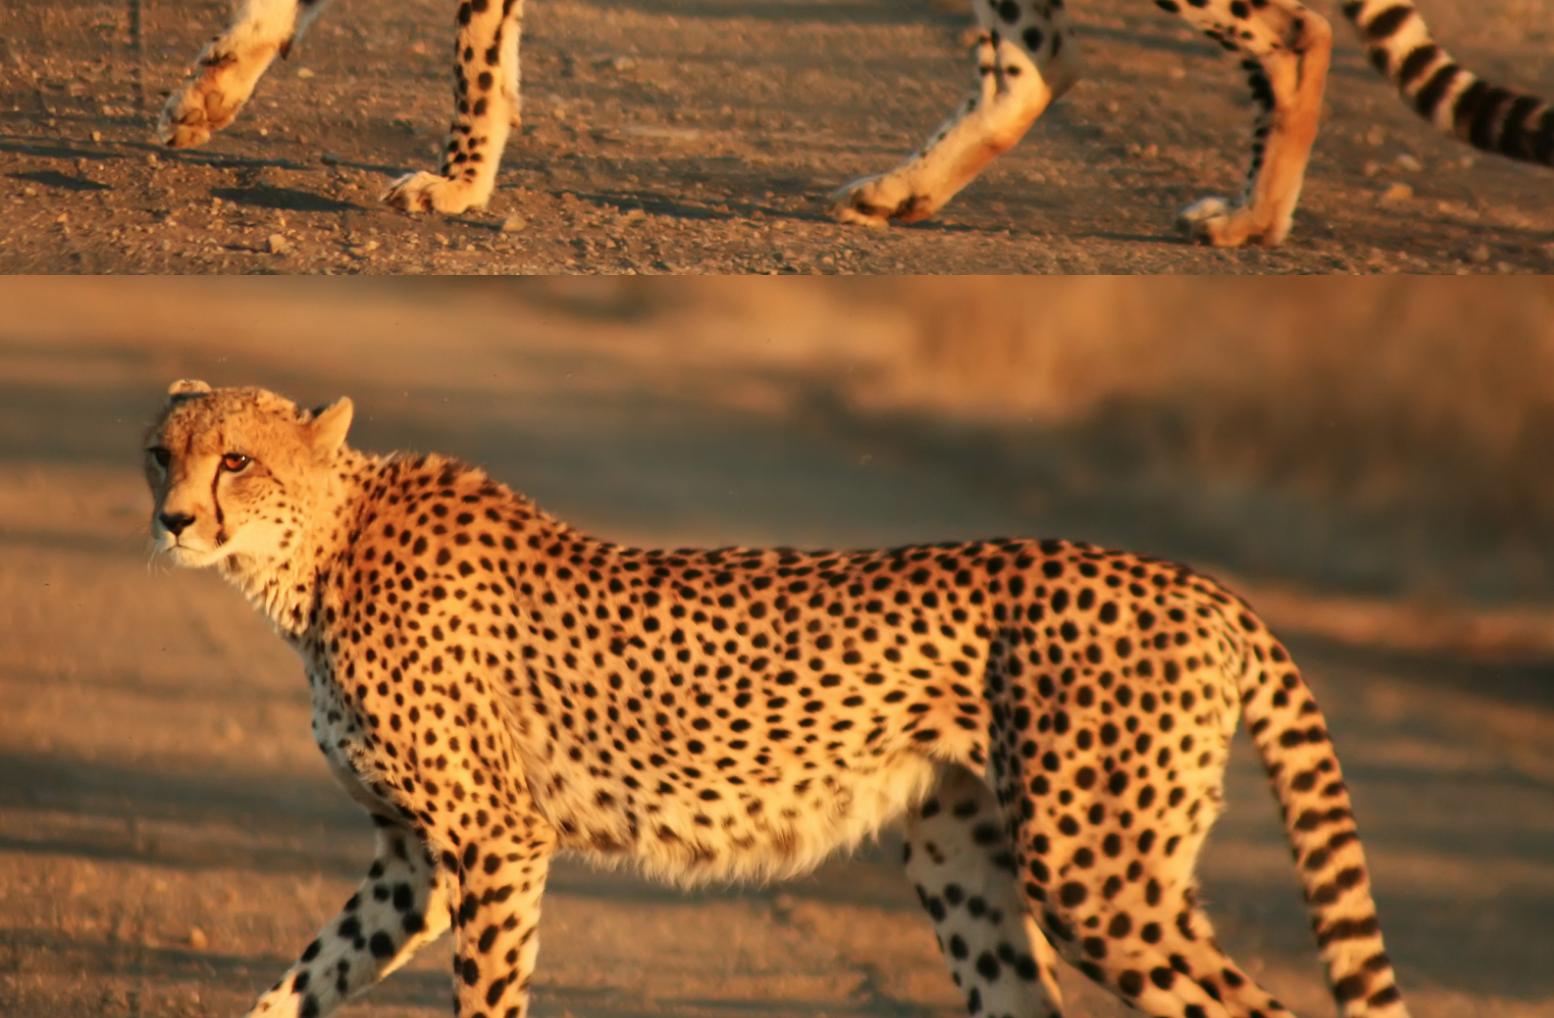
\includegraphics[scale=0.3]{TSP_OUTPUT.png}
\caption{Shows the scrumbled image after applying TSP}
\end{figure}
The problem in Figure 4 is deciding the first row. To decide which is the best cut I just searched for maximum distance between two neighbours and take the first one as the start.Here is the code that should be added the the previous one to fix the problem:
\begin{lstlisting}[language=Python]
#Find the Best Cut
maxvalue=0
maxindex=-1
for i in range(len(plan)-1):
    dist = np.linalg.norm(plan[i]-plan[i+1])
    if (dist>maxvalue):
        maxvalue = dist
        maxindex=i

lst2=output[maxindex:] + output[:maxindex]
\end{lstlisting}
\begin{figure}[H]
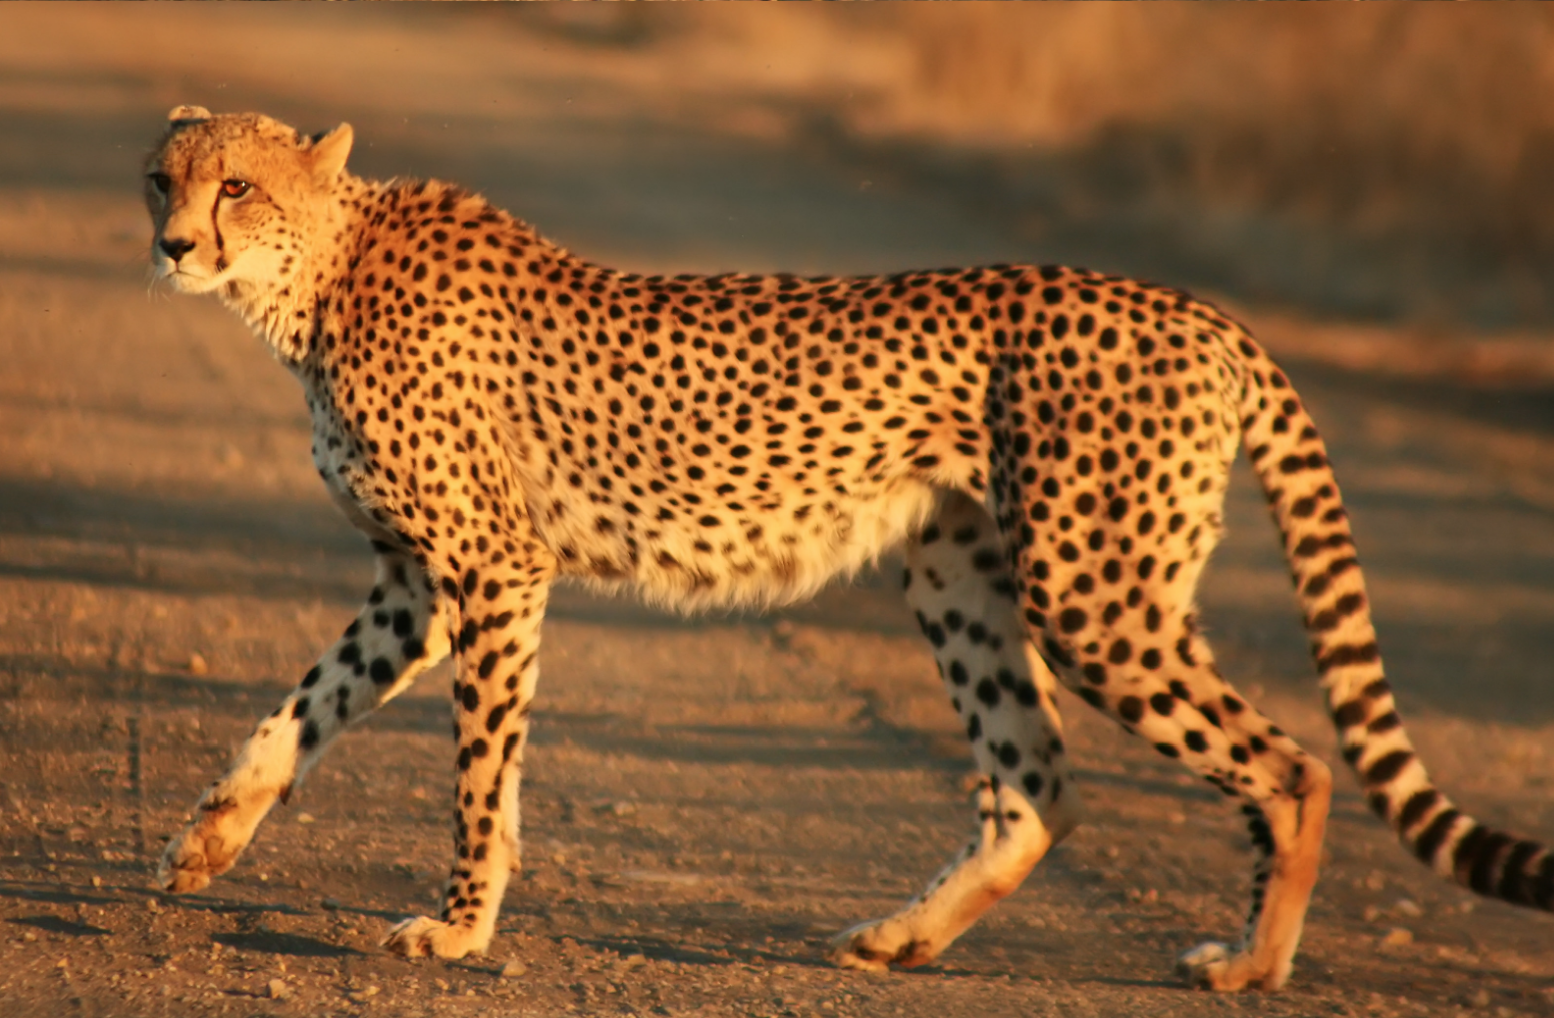
\includegraphics[scale=0.3]{TSP_OUTPUT_Perfect.png}
\caption{Image after optimizing the start point}
\end{figure}
Just for fun I applied the same software in the second image and I got the following result:
\begin{figure}[H]
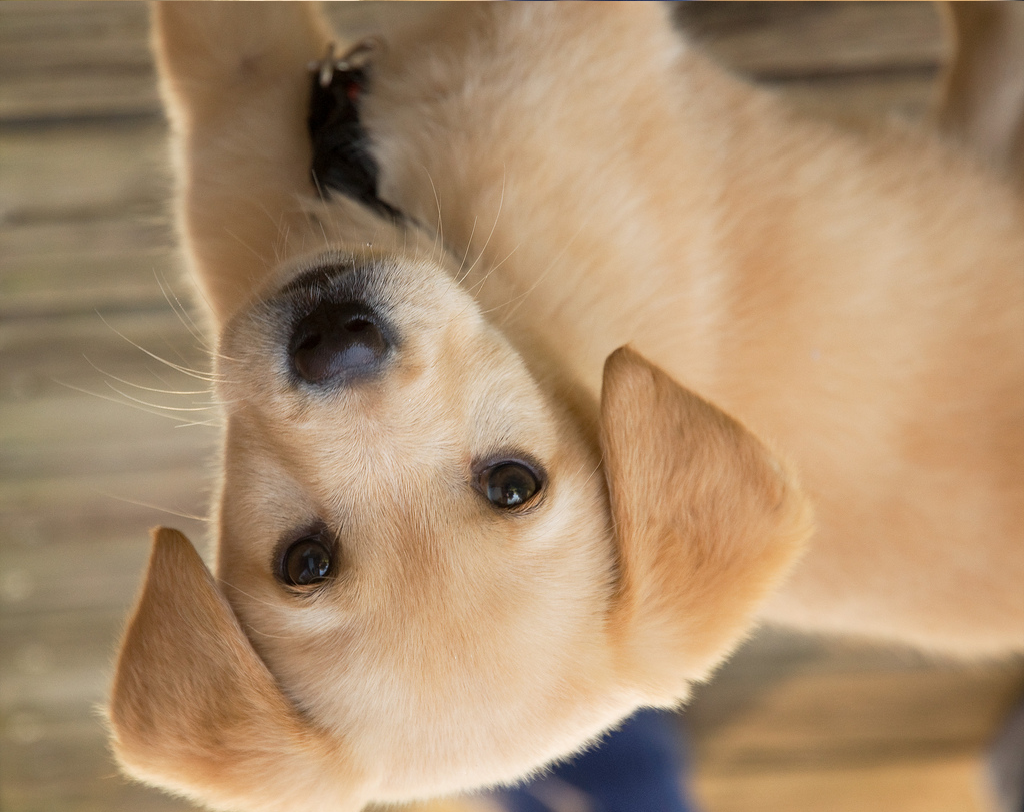
\includegraphics[scale=0.4]{TSP_OUTPUT2.png}
\caption{Image 2 after recovering using TSP with optimized start point}
\end{figure}
\section*{Seventh Question}


For this question I used mysql.And I used the following steps to achieve the pivot table using sql 
\begin{enumerate}
\item Created table in the database using the following code:
\begin{lstlisting}[language=SQL]
CREATE TABLE `census` (`State` varchar(50) DEFAULT NULL,  `House_id` varchar(50) DEFAULT NULL,  `Weight` varchar(50) DEFAULT NULL,  `House_relation` varchar(50) DEFAULT NULL,  `Sex` varchar(50) DEFAULT NULL,  `Age` varchar(50) DEFAULT NULL,  `Race` varchar(50) DEFAULT NULL,  `Marriage` varchar(50) DEFAULT NULL,  `Education` varchar(50) DEFAULT NULL,  `Ancestry` varchar(50) DEFAULT NULL,  `Language` varchar(50) DEFAULT NULL,  `Employment_status` varchar(50) DEFAULT NULL,  `Traveltime` varchar(50) DEFAULT NULL,  `Industry` varchar(50) DEFAULT NULL,  `Occupation` varchar(50) DEFAULT NULL,  `Hours` varchar(50) DEFAULT NULL,  `Weeks` varchar(50) DEFAULT NULL,  `Salary` varchar(50) DEFAULT NULL,  `Income` varchar(50) DEFAULT NULL,  `Earnings` int(20) DEFAULT NULL)
\end{lstlisting}
\item After that I loaded the data into the table using the following code : 
\begin{lstlisting}[language=SQL]
#Show the directory that mysql can accept files from
SHOW VARIABLES LIKE "secure_file_priv";
LOAD DATA INFILE '/var/lib/mysql-files/extract_large.csv' 
INTO TABLE census
FIELDS TERMINATED BY ';'
\end{lstlisting}

\item At the end, I used the following code to generate the pivot table :
\begin{lstlisting}[language=SQL]
SELECT Sex,Education,avg(Earnings)
FROM census
group by Sex,Education
\end{lstlisting}
Which clearly find the average earning for each set of (Sex,Education)
\end{enumerate}
Here is the output table :\\
\begin{tabular}{|c|c|c|}
\hline
Sex&Education&Avg(Earnings)\\ \hline
1&00&0.0000\\ \hline 
1&01&3436.9163\\ \hline 
1&02&1018.5143\\ \hline 
1&03&5719.2300\\ \hline 
1&04&4585.9244\\ \hline 
1&05&7892.1493\\ \hline 
1&06&8702.8604\\ \hline 
1&07&10341.6579\\ \hline 
1&08&16704.6764\\ \hline 
1&09&22399.7355\\ \hline 
1&10&26831.3657\\ \hline 
1&11&29900.6087\\ \hline 
1&12&35249.8174\\ \hline 
1&13&52814.0881\\ \hline 
1&14&63902.4224\\ \hline 
1&15&97160.4380\\ \hline 
1&16&69790.5412\\ \hline 
2&00&0.0000\\ \hline 
2&01&1358.9230\\ \hline 
2&02&386.2795\\ \hline 
2&03&1996.0910\\ \hline 
2&04&1656.8459\\ \hline 
2&05&3048.7202\\ \hline 
2&06&3878.9171\\ \hline 
2&07&4711.3237\\ \hline 
2&08&7794.4182\\ \hline 
2&09&10865.3802\\ \hline 
2&10&15102.8411\\ \hline 
2&11&16310.1780\\ \hline 
2&12&20708.8457\\ \hline 
2&13&27804.7783\\ \hline 
2&14&35058.9334\\ \hline 
2&15&44529.5096\\ \hline 
2&16&44325.0832\\ \hline 
\end{tabular}
\begin{thebibliography}{9}
\bibitem{1}
\href{https://joernhees.de/blog/2015/08/26/scipy-hierarchical-clustering-and-dendrogram-tutorial/}{SciPy Hierarchical Clustering and Dendrogram Tutorial}
\end{thebibliography}
\textbf{Note:}All .py,.ipython,.tex,.pdf etc.. exist on \href{URL}{github}
\begin{center}
\textbf{E.O.F}
\end{center}



\end{document}
